\documentclass[__main__.tex]{subfiles}

\begin{document}

\qtitle{О}{13}
Поле диполя Герца, волновая зона, интенсивность излучения, диаграмма направленности.\\ 

\begin{wrapfigure}{R}{.25\linewidth}
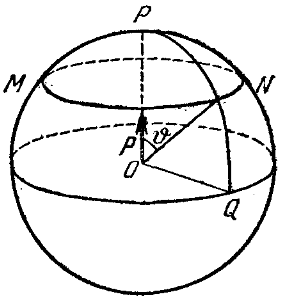
\includegraphics[width=1\linewidth]{О-13_1}
\caption{}
\llabel{o13:fig-sp}
\end{wrapfigure}

\begin{definition}
\emph{Диполь Герца} -- точечный диполь, дипольный момент которого колеблется с течением времени. 
\end{definition}
Диполь Герца является простейшей системой, излучающей электромагнитные волны. Опишем поле излучения диполя с моментом $\vec{p}$ в среде с диэлектрической и магнитной проницаемостями $\varepsilon$ и $\mu$. Начало координат положим в точке нахождения диполя. Если бы $\vec{p}=\overline{const}$, то вектор электрической индукции $\vec{D}$ имел бы вид:
\begin{gather}
\vec{D}=\frac{3\left<\vec{p},\vec{r}\right>}{r^5}\vec{r}-\frac{\vec{p}}{r^3}
\llabel{o13:static}
\end{gather}
изменим выражение (\lref{o13:static}) для случая переменного $\vec{p}$: на малых расстояниях $\vec{D}$ должен быть равен значению из электростатики, следовательно, убывать пропорционально $r^3$. К этому выражению добавим слагаемые, зависящие от производных $\vec{p}$ по времени и убывающие медленнее. Следовательно, будем искать $\vec{D}$ в виде:
\begin{gather}
\llabel{o13:mans}
\vec{D}
=
\left(
\frac{3\left<\vec{p},\vec{r}\right>}{r^5}\vec{r}-\frac{\vec{p}}{r^3}
\right)
+
\left(
a\frac{\left<\dot{\vec{p}},\vec{r}\right>}{vr^4}+b\frac{\dot{\vec{p}}}{vr^2}
\right)
+
\left(
f\frac{\left<\ddot{\vec{p}},\vec{r}\right>}{v^2r^3}\vec{r}+h\frac{\ddot{\vec{p}}}{v^2r}
\right),
\end{gather}
где $a$, $b$, $c$, $d$ -- безразмерные постоянные. Предполагаются, что производные по $\vec{p}$ берутся в момент времени $t'=t-r/v$ (если $t$ -- момент времени, когда волна достигла $\vec{r}$, то $t'$ момент ее выхода из диполя). Найдем коэффициенты (\lref{o13:mans}) из уравнений Максвелла:
\begin{flalign*}
\nabla\vec{D}
=&
-2(b+1)\frac{\left<\partial_{t}\vec{p},\vec{r}\right>}{vr^4}
-(a+b+f+h)\frac{\left<\partial_{t}^2\vec{p},\vec{r}\right>}{v^2r^3}
-(f+h)\frac{\left<\partial_{t}^3\vec{p},\vec{r}\right>}{v^3r^2}
=\\
=&
0
\end{flalign*}
т.к. $\partial_{t}\vec{p}$, $\partial_{t}^2\vec{p}$, $\partial_{t}^3\vec{p}$ независимы, то коэффициенты этого выражения должны обращаться в нуль. Получим:
\begin{gather}
b=-1,
\qquad
h=-f,
\qquad
a-2f=1,
\end{gather}
Найдем магнитное поле $\vec{H}$ при помощи теоремы Гаусса для определения $a$ и $f$:
\begin{gather*}
\oint_{l}\vec{H}d\vec{l}=\frac{1}{c}\oiint_{S}\left<\vec{D},\vec{n}\right>dS,
\end{gather*}
где $S$ -- сфера, ограниченная окружностью $MN$, см. Рис. \lref{o13:fig-sp}. $l$ -- $MN$. Получим:
\begin{gather}
\frac{1}{c}\oiint_{S}\left<\vec{D},\vec{n}\right>dS
=
\left(\frac{2p}{r}+\frac{a-1}{v}\dot{p}\right)\pi\sin^2\theta,
\end{gather}
Получим $\vec{H}$:
\begin{gather}
\vec{H}
=
\frac{\partial_{t}\vec{p}\times\vec{r}}{cr^3}+\frac{a-1}{2cvr^2}\partial_{t}^2\vec{p}\times\vec{r},
\end{gather}
несложно убедиться, что $\nabla\vec{H}=0$ выполняется. Теперь определим $a$ через последнее уравнение Максвелла:
\begin{gather}
\nabla\times\vec{D}=-\frac{\varepsilon\mu}{c}\partial_{t}\vec{H},
\end{gather}
получим:
\begin{gather}
\nabla\times\vec{D}
=
(a-3)\frac{\partial_{t}\vec{p}\times\vec{r}}{vr^4}
-\frac{\partial_{t}^2\vec{p}\times\vec{r}}{v^2r^3}
-f\frac{\partial_{t}^3\vec{p}\times\vec{r}}{v^3r^2},
\end{gather}
с другой стороны с учетом $c^2=\varepsilon\mu{v^2}$ получим:
\begin{gather}
-\frac{\varepsilon\mu}{c}\partial_{t}\vec{H}
=
-\frac{\partial_{t}^2\vec{p}\times\vec{r}}{v^2r^3}
-\frac{a-1}{2v^3r^2}\partial_{t}^3\vec{p}\times\vec{r}.
\end{gather}
Из этих соотношений получим $a=3$, $f=1$. Т.е. окончательный вид поля диполя Герца:
\begin{flalign}
\begin{split}
&
\vec{D}
=
\left[ \frac{3\left<\vec{p},\vec{r}\right>}{r^5}\vec{r}-\frac{\vec{p}}{r^3} \right]_{t-\frac{r}{v}}
+
\left[ \frac{3\left<\partial_{t}\vec{p},\vec{r}\right>}{vr^4}-\frac{\partial_{t}\vec{p}}{vr^2} \right]_{t-\frac{r}{v}}
+
\left[ \frac{\left<\partial_{t}^2\vec{p},\vec{r}\right>}{v^2r^3}\vec{r}-\frac{\partial_{t}^2\vec{p}}{v^2r} \right]_{t-\frac{r}{v}},
\\
&
\vec{H}
=
\left.\frac{1}{cr^3}\partial_{t}\vec{p}\times\vec{r}\right|_{t-\frac{r}{v}}
+
\left.\frac{1}{cvr^2}\partial_{t}^2\vec{p}\times\vec{r}\right|_{t-\frac{r}{v}},
\end{split}
\llabel{o13:final}
\end{flalign}

\begin{wrapfigure}{R}{.25\linewidth}
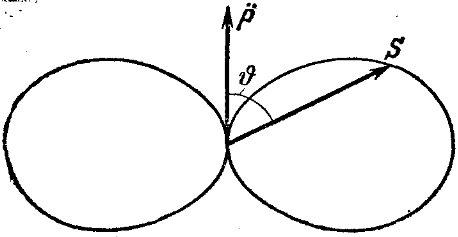
\includegraphics[width=1\linewidth]{О-13_2}
\caption{}
\llabel{o13:fig-diag}
\vspace{5mm}
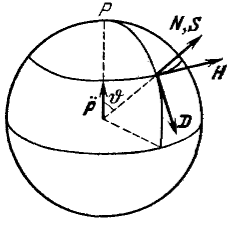
\includegraphics[width=1\linewidth]{О-13_3}
\caption{}
\llabel{o13:fig-sp1}
\end{wrapfigure}

Индекс $t-\frac{r}{v}$ подразумевает, что значения дипольного момента и его производных берется в момент времени $t-\frac{r}{v}$. Поля (\lref{o13:final}) можно разложить в зависимости от скорости убывания в зависимости от расстояния $r$. Заметим, что в (\lref{o13:final}) некоторые слагаемые увеличением $r$ убывают гораздо быстрее с чем остальные, т.е. на достаточно большом удалении от диполя этими слагаемыми можно пренебречь. Область, в которой мы пренебрегаем этими слагаемыми называют \textbf{волновой зоной} диполя, а само поле в этой зоне можно записать так:
\begin{flalign}
\begin{split}
&
\vec{D}_\text{B}
=
\left[ \frac{\left<\partial_{t}^2\vec{p},\vec{r}\right>}{v^2r^3}\vec{r}-\frac{\partial_{t}^2\vec{p}}{v^2r} \right]_{t-\frac{r}{v}}
=
\frac{1}{v^2r^3}
\left.
\partial_{t}^2\vec{p}\times\vec{r}\times\vec{r}
\right|_{t-\frac{r}{v}},
\\
&
\vec{H}_\text{B}
=
\left.\frac{1}{cvr^2}\partial_{t}^2\vec{p}\times\vec{r}\right|_{t-\frac{r}{v}},
\end{split}
\end{flalign}
Следовательно:
\begin{gather}
\vec{D}_\text{B}=\frac{c}{v}\vec{H}\times\vec{e}_r,
\qquad
\vec{H}_\text{B}=\frac{v}{c}\vec{e}_r\times\vec{D},
\end{gather}
где $\vec{e}_r=\frac{\vec{r}}{r}$. Получим, что $\vec{r}$, $\vec{D}$, $\vec{H}$ -- ортогональная система векторов. Вектор Поинтинга $\vec{S}$ плотности потока энергии примет вид:
\begin{gather}
\vec{S}
=
\frac{c}{4\pi\varepsilon}\vec{D}\times\vec{H}
=
\frac{c^2}{4\pi\varepsilon{v}}H^2\vec{e}_r
=
\frac{\sin^2\theta}{4\pi\varepsilon{v^3r^2}}\left.\partial_{t}^2\vec{p}\right|_{t-\frac{r}{v}}\vec{e}_{r},
\end{gather}
где $\theta=\angle(\partial_{t}^2,\vec{r})$. \emph{Диаграмму направленности} диполя Герца см. на Рис. \lref{o13:fig-diag}.

Таким образом получим, что поток энергии направлен \emph{вдоль радиуса} и его плотность \emph{обратно пропорциональна квадрату расстояния $r$}. Излучение не \emph{изотропно}, в направлении $\partial_{t}^2\vec{p}$ оно отсутствует.

Найдем \textbf{интегральную мощность излучения $\frac{dE}{dt}$}: для этого проинтегрируем $S=||\vec{S}||$ по сфере радиуса $r$:
\begin{gather}
\frac{dE}{dt}
=
\oiint\limits_{S^2_r}S\cdot{2\pi r^2\sin\theta{d\theta}}
=
\frac{2}{3\varepsilon{v^3}}\left(\partial_{t}^2\vec{p}\right)^2_{t-\frac{r}{v}}
\end{gather}

\end{document}
